\documentclass[12pt]{article}

\usepackage{fontspec}
\usepackage{amsmath, amssymb, amsfonts}
\usepackage{graphicx}
\usepackage{hyperref}
\usepackage{color}
\usepackage{geometry}
\geometry{a4paper}

\usepackage{tikz}
\usetikzlibrary{calc, positioning}

\begin{document}

	\vspace{3em}
	\begin{center}
			{\Large Exercices : domaines et images des fonctions}
	\end{center}
	
	\vspace{2em}
	
	\begin{enumerate}
		\item 
			Soit les ensemble $I$ et $J$ et la notation formelle de fonction suivante :
				\begin{equation*}
					f : I \mapsto J : x \mapsto f(x)
				\end{equation*}
			Quel est le nom de la fonction ? Quel est le domaine ? Quelle est l'image ?
			
		\item 
			Soit la fonction $f$ définie par $f(x) = \frac{1}{x}$. Ecris cette fonction en utilisant la bonne notation (fais attention au domaine et à l'image).
			
		\item
			Soit la fonction $f$ définie par $f(x) = 3x² - x + 6$. Remplis le tableau suivant~:
			\begin{center}
				\begin{tabular}{c|c|c|c|c|c|c}
					$x$ & 0 & 1 & 2 & 3 & 4 & 5 \\
					\hline
					$f(x)$ & \hspace{1em} & \hspace{1em} & \hspace{1em} & \hspace{1em} & \hspace{1em} & \hspace{1em}
				\end{tabular}
			\end{center}
		
		\item 
			Ecris le domaine des fonctions suivantes :
			\begin{enumerate}
				\item $f(x) = \sqrt{x}$
				\item $g(x) = \frac{1}{x}$
				\item $h(x) = \frac{1}{\sqrt{4 - x^2}}$
				\item $i(x) = \frac{1}{x^2 - 1}$
				\item $j(x) = \sqrt[3]{x}$
				\item $k(x) = \frac{\sqrt{x + 1}}{x - 2}$
				\item $l(x) = \frac{1}{|x|}$
			\end{enumerate}
		
		\item 
			Soit les graphiques représentés dans les repères orthonormés ci-dessous. Pour chacun des graphiques, détermine si c'est la graphique d'une fonction et justifie~:
			\begin{figure}
				\begin{minipage}[t]{0.5\textwidth}
					\centering
					\begin{tikzpicture}
						\begin{axis}[
							xlabel={$x$},
							ylabel={$y$},
							xmin=-2,
							xmax=2,
							ymin=0,
							ymax=4,
							axis lines=middle,
							]
							\addplot [domain=-2:2, samples=100] {x^2};
						\end{axis}
					\end{tikzpicture}
					\caption{$f(x)$}
				\end{minipage}%
				\begin{minipage}[t]{0.5\textwidth}
					\centering
					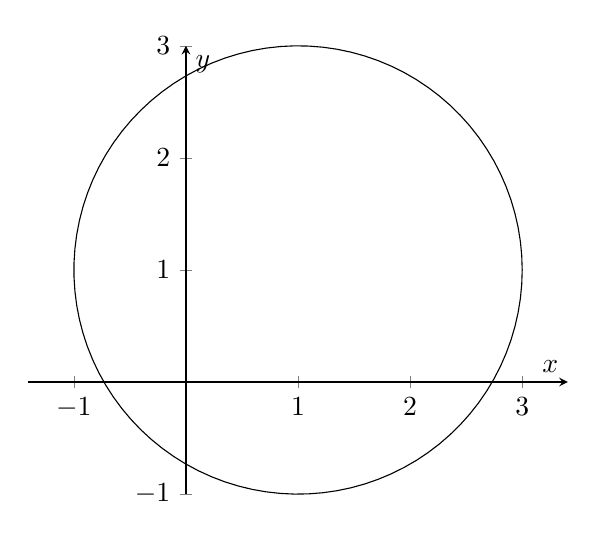
\begin{tikzpicture}
						\begin{axis}[
							axis equal,
							xlabel={$x$},
							ylabel={$y$},
							xmin=-1,
							xmax=3,
							ymin=-1,
							ymax=3,
							axis lines=middle,
							]
							\addplot [domain=0:360, samples=100] ({1 + 2*cos(x)}, {1 + 2*sin(x)});
						\end{axis}
					\end{tikzpicture}
					\caption{$g(x)$}
				\end{minipage}
			\end{figure}

	\end{enumerate}
	
\end{document}